\section{Relative Performance Identity}\label{RPIsection} 

\subsection{Advantage-функция}

Введём ещё одну <<оценочную функцию>>, уже больше из соображений удобства (просто везде вылезает):

\begin{definition} 
Для данного MDP \emph{Advantage-функцией} политики $\pi$ называется
\begin{equation}\label{advantage}
A^\pi(s, a) \coloneqq Q^\pi(s, a) - V^\pi(s)
\end{equation}
\end{definition}

\begin{proposition}\label{pr:advantageiszero}
Для любой политики $\pi$ и любого состояния $s$:
$$\E_{\pi(a \mid s)} A^\pi(s, a) = 0$$
\beginproof
\begin{align*}
\E_{\pi(a \mid s)} A^\pi(s, a) &= \E_{\pi(a \mid s)} Q^\pi(s, a) - \E_{\pi(a \mid s)} V^\pi(s) = \\
\{ \text{$V^\pi$ не зависит от $a$} \} &= \E_{\pi(a \mid s)} Q^\pi(s, a) - V^\pi(s) = \\
\{ \text{связь $V$ через $Q$ \eqref{VQ}} \} &= V^\pi(s) - V^\pi(s) = 0   \tagqed
\end{align*}
\end{proposition}

\begin{proposition}
\label{adv_is_positive}
Для любой политики $\pi$ и любого состояния $s$:
$$\max_a A^\pi(s, a) \ge 0$$
\end{proposition}

Advantage --- это, если угодно, <<центрированная>> Q-функция. У неё есть важная интуиция: насколько хорошо (<<удачно>>) для политики $\pi$ выбрать в состоянии $s$ действие $a$? Мы знаем, что вообще в среднем она набирает из данного состояния $V^\pi(s)$, но какой-то выбор действий даст в итоге награду больше $V^\pi(s)$, а какой-то меньше. Если $A^\pi(s, a) \HM> 0$ --- действие $a$ <<лучше среднего>> для нашей текущей политики в состоянии $s$, меньше нуля --- хуже. И интуиция, что первые надо выбирать чаще, а вторые --- реже, нас не обманывает.

\subsection{Relative Performance Identity (RPI)}

Мы сейчас докажем одну очень интересную лемму, которая не так часто нам будет нужна в будущем, но которая прям открывает глаза на мир. Нам понадобится следующий трюк (\emph{telescoping sums}): для любой последовательности $a_t$, т.~ч. $\lim\limits_{t \to \infty} a_t \HM= 0$, верно
$$\sum_{t \ge 0}^\infty \left( a_{t+1} - a_t \right) = -a_0$$

Мы применим его к value-функции следующим образом:
\begin{proposition}

\begin{equation}\label{trick}
-V^{\pi}(s_0) = \sum_{t \ge 0} \left[ \gamma^{t+1} V^{\pi}(s_{t+1}) - \gamma^{t} V^{\pi}(s_t) \right]
\end{equation}

\begin{proof} Достаточно проверить, что $\lim\limits_{t \to \infty} \gamma^{t} V^{\pi}(s_t) \HM= 0$, что верно в силу ограниченности V-функции в рамках рассматриваемых ограничений на MDP. Если в игре конечное число шагов, не сокращающееся слагаемое $V^\pi(s)$ есть функция ценности терминального состояния, которая по определению равна нулю.
\end{proof}
\end{proposition}

Лемма показывает, как связан performance $J(\pi) = V^\pi(s_0)$ двух разных стратегий. В общем виде лемма сравнивает V-функции двух стратегий в одном состоянии:

\begin{theoremBox}[label=th:rpi]{Relative Performance Identity}
Для любых двух политик $\textcolor{ChadBlue}{\pi_1}$, $\textcolor{ChadPurple}{\pi_2}$:
\begin{equation}\label{RPI}
\textcolor{ChadPurple}{V^{\pi_2}}(s) - \textcolor{ChadBlue}{V^{\pi_1}}(s) = \E_{\textcolor{ChadPurple}{\Traj \sim \pi_2} \mid s_0 = s} \sum_{t \ge 0} \gamma^t \textcolor{ChadBlue}{A^{\pi_1}}(s_t, a_t)
\end{equation}
\beginproof
\begin{align*}
\textcolor{ChadPurple}{V^{\pi_2}}(s) - \textcolor{ChadBlue}{V^{\pi_1}}(s) &= \E_{\textcolor{ChadPurple}{\Traj \sim \pi_2} \mid s_0 = s} \sum_{t \ge 0} \gamma^t r_t - \textcolor{ChadBlue}{V^{\pi_1}}(s) = \\
&= \E_{\textcolor{ChadPurple}{\Traj \sim \pi_2} \mid s_0 = s} \left[\sum_{t \ge 0} \gamma^t r_t - \textcolor{ChadBlue}{V^{\pi_1}}(s_0) \right] = \\
\{ \text{трюк \eqref{trick}} \} &= \E_{\textcolor{ChadPurple}{\Traj \sim \pi_2} \mid s_0 = s} \left[\sum_{t \ge 0} \gamma^t r_t + \sum_{t \ge 0} \left[ \gamma^{t+1} \textcolor{ChadBlue}{V^{\pi_1}}(s_{t+1}) - \gamma^t \textcolor{ChadBlue}{V^{\pi_1}}(s_t) \right] \right] = \\
\{ \text{перегруппируем слагаемые} \} &= \E_{\textcolor{ChadPurple}{\Traj \sim \pi_2} \mid s_0 = s} \sum_{t \ge 0} \gamma^t \left( r_t + \gamma \textcolor{ChadBlue}{V^{\pi_1}}(s_{t+1}) - \textcolor{ChadBlue}{V^{\pi_1}}(s_t) \right) = \\
\{ \text{фокус $\E_x f(x) = \E_x \E_x f(x)$} \} &= \E_{\textcolor{ChadPurple}{\Traj \sim \pi_2} \mid s_0 = s} \sum_{t \ge 0} \gamma^t \left( r_t + \gamma \E_{s_{t+1}} \textcolor{ChadBlue}{V^{\pi_1}}(s_{t+1}) - \textcolor{ChadBlue}{V^{\pi_1}}(s_t) \right) = \\
\{ \text{выделяем Q-функцию \eqref{QV}} \} &= \E_{\textcolor{ChadPurple}{\Traj \sim \pi_2} \mid s_0 = s} \sum_{t \ge 0} \gamma^t \left( \textcolor{ChadBlue}{Q^{\pi_1}}(s_t, a_t) - \textcolor{ChadBlue}{V^{\pi_1}}(s_t) \right) \\
\{ \text{по определению \eqref{advantage}} \} &= \E_{\textcolor{ChadPurple}{\Traj \sim \pi_2} \mid s_0 = s} \sum_{t \ge 0} \gamma^t \textcolor{ChadBlue}{A^{\pi_1}}(s_t, a_t)   \tagqed
\end{align*}
\end{theoremBox}

Мы смогли записать наш функционал как мат.ожидание по траекториям, сгенерированным одной политикой, по оценочной функции другой стратегии. Грубо говоря, мы можем награду заменить Advantage-функцией произвольной другой стратегии, и это сдвинет оптимизируемый функционал на константу! Прикольно.

\subsection{Policy Improvement}

\begin{definition}
Будем говорить, что стратегия $\pi_2$ <<\emph{не хуже}>> $\pi_1$ (запись: $\pi_2 \succeq \pi_1$), если $\forall s \colon$
$$V^{\pi_2}(s) \ge V^{\pi_1}(s),$$
и \emph{лучше} (запись: $\pi_2 \succ \pi_1$), если также найдётся $s$, для которого неравенство выполнено строго:
$$V^{\pi_2}(s) > V^{\pi_1}(s)$$
\end{definition}

Мы ввели частичный порядок на множестве стратегий (понятно, что можно придумать две стратегии, которые будут <<не сравнимы>>: когда в одном состоянии одна будет набирать больше второй, в другом состоянии вторая будет набирать больше первой).

Зададимся следующим вопросом. Пусть для стратегии $\pi_1$ мы знаем оценочную функцию $Q^{\pi_1}$; тогда мы знаем и $V^{\pi_1}$ из VQ уравнения \eqref{VQ} и $A^{\pi_1}$ по определению \eqref{advantage}. Давайте попробуем построить $\pi_2 \succ \pi_1$. Интуицию построения попробуем <<подсмотреть>> из леммы RPI: мы не очень понимаем, как выбор тех или иных действий в состоянии влияет на структуру траектории $p(\Traj \mid \pi_2)$, но можем определить, какие пары ($s, a$) в принципе могут встречаться в этих траекториях. Что, если $\pi_2$ во всех состояниях $s$ выбирает только действия $a$, на которых $A^{\pi_1}(s, a) \ge 0$ неотрицателен, то есть что, если в формуле \eqref{RPI} под интегралом справа стоят только неотрицательные слагаемые? Такие действия во всех состояниях есть, поскольку Advantage <<центрирован>> к нулю --- утв. \ref{adv_is_positive}. Тогда и интеграл в правой части RPI точно будет неотрицателен, каковыми бы ни были траектории, порождаемые $\pi_2$, и тогда $V^{\pi_2}(s) \HM- V^{\pi_1}(s) \HM\ge 0$ для всех $s$.

Покажем более <<классическим>> способом, что стратегии $\pi_2$ достаточно лишь в среднем выбирать действия, дающие неотрицательный Advantage стратегии $\pi_1$, чтобы быть не хуже.

\begin{theoremBox}[label=th:policyimprovement]{Policy Improvement}
Пусть стратегии $\textcolor{ChadBlue}{\pi_1}$ и $\textcolor{ChadPurple}{\pi_2}$ таковы, что для всех состояний $s$ выполняется:
$$\E_{\textcolor{ChadPurple}{\pi_2}(a \mid s)} \textcolor{ChadBlue}{Q^{\pi_1}}(s, a) \ge \textcolor{ChadBlue}{V^{\pi_1}}(s),$$
или, в эквивалентной форме:
$$\E_{\textcolor{ChadPurple}{\pi_2}(a \mid s)} \textcolor{ChadBlue}{A^{\pi_1}}(s, a) \ge 0.$$
Тогда $\textcolor{ChadPurple}{\pi_2} \succeq \textcolor{ChadBlue}{\pi_1}$; если хотя бы для одного $s$ неравенство выполнено строго, то $\textcolor{ChadPurple}{\pi_2} \succ \textcolor{ChadBlue}{\pi_1}$.
\begin{proof}
Покажем, что $\textcolor{ChadPurple}{V^{\pi_2}}(s) \ge \textcolor{ChadBlue}{V^{\pi_1}}(s)$ для любого $s$:
\begin{align*}
\textcolor{ChadBlue}{V^{\pi_1}}(s) = \{ \text{связь VQ \eqref{VQ}} \} &= \E_{\textcolor{ChadBlue}{\pi_1}(a \mid s)} \textcolor{ChadBlue}{Q^{\pi_1}}(s, a) \le \\
= \{ \text{по построению $\textcolor{ChadPurple}{\pi_2}$} \} &= \E_{\textcolor{ChadPurple}{\pi_2}(a \mid s)} \textcolor{ChadBlue}{Q^{\pi_1}}(s, a) = \\
= \{ \text{связь QV \eqref{QV}} \} &= \E_{\textcolor{ChadPurple}{\pi_2}(a \mid s)} \left[ r + \gamma \E_{s'} \textcolor{ChadBlue}{V^{\pi_1}}(s') \right] \le \\
\le \{ \text{раскручиваем цепочку далее} \} &\le \dots \le \E_{\textcolor{ChadPurple}{\Traj \sim \pi_2} \mid s_0 = s} \sum_{t \ge 0} \gamma^t r_t = \\
= \{ \text{по определению \eqref{Vdefinition}} \} &= \textcolor{ChadPurple}{V^{\pi_2}}(s)
\end{align*}
Если для какого-то $s$ неравенство из условия теоремы было выполнено строго, то для него первое неравенство в этой цепочке рассуждений выполняется строго, и, значит, $\textcolor{ChadPurple}{V^{\pi_2}}(s) > \textcolor{ChadBlue}{V^{\pi_1}}(s)$.
\end{proof}
\end{theoremBox}

% TODO: пример

Что означает эта теорема? Знание оценочной функции позволяет улучшить стратегию. В частности, мы можем это сделать \emph{жадно}, взяв детерминированную $\pi_2$:
$$\pi_2(s) \coloneqq \argmax\limits_{a} Q^{\pi_1}(s, a) = \argmax\limits_{a} A^{\pi_1}(s, a)$$

% \begin{proposition}
% Пусть $\pi_2$ такова, что $\forall s, a \colon \pi_2(a \mid s) > 0 \Rightarrow a \in \Argmax\limits_a A^{\pi_1}(s, a)$. Тогда $\pi_2 \succeq \pi_1$.
% \end{proposition}

Тогда, какой бы ни была $\pi_1$, в силу утверждения \ref{adv_is_positive}, гласящего, что $\max\limits_a A^{\pi_1}(s, a) \ge 0$, мы попадаем под теорему \ref{th:policyimprovement} и имеем гарантии $\pi_2 \succeq \pi_1$. Мы так не получим, конечно же, <<за один ход>> сразу оптимальную стратегию, поскольку выбор $\pi_2(a \mid s)$ сколько угодно хитро может изменить распределение траекторий, но тем не менее.

\needspace{15\baselineskip}
\begin{example}
Попробуем улучшить стратегию $\pi$ из примера \ref{ex:vfunction}, $\gamma = 0.8$. Например, в состоянии C она выбирает \colorsquare{ChadRed} с вероятностью 1 и получает -1; попробуем посчитать $Q^{\pi}(s \HM= C, \colorsquare{ChadBlue})$:
$$
Q^{\pi}(s = C, \colorsquare{ChadBlue}) = 0.2\gamma V^{\pi}(C) + 0.8 \gamma V^{\pi}(B)
$$
\needspace{13\baselineskip}
\begin{wrapfigure}{r}{0.45\textwidth}
\vspace{-0.8cm}
\centering
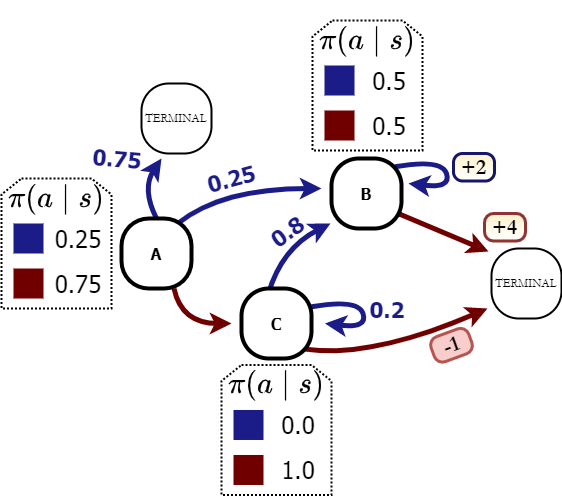
\includegraphics[width=0.4\textwidth]{Images/Value.png}
%\vspace{-0.4cm}
\end{wrapfigure}
Подставляя ранее подсчитанные $V^{\pi}(C) \HM= -1, V^{\pi}(B) \HM= 5$, видим, что действие \colorsquare{ChadBlue} принесло бы нашей стратегии $\pi$ куда больше -1, а именно $Q^{\pi}(s = C, \colorsquare{ChadBlue}) \HM= 3.04$. Давайте построим $\pi_2$, скопировав $\pi$ в A и B, а в C будем с вероятностью 1 выбирать \colorsquare{ChadBlue}.

Что говорит нам теория? Важно, что она не даёт нам значение $V^{\pi_2}(C)$; в частности, нельзя утверждать, что $Q^{\pi_2}(s = C, \colorsquare{ChadBlue}) \HM= 3.04$, и повторение вычислений подтвердит, что это не так. Однако у нас есть гарантии, что, во-первых, $V^{\pi_2}(C) \HM> V^{\pi_1}(C)$ строго, во-вторых, что мы не <<сломали>> стратегию в других состояниях: во всех остальных состояниях гарантированно $V^{\pi_2}(s) \HM\ge V^{\pi_1}(s)$. Для Q-функции, как можно показать, выполняются аналогичные неравенства.
\end{example}

Что, если для некоторой $\pi_1$ мы <<не можем>> провести Policy Improvement? Под этим будем понимать, что мы не можем выбрать $\pi_{2}$ так, что $\E_{\pi_{2}(a \mid s)} Q^{\pi_{1}}(s, a) \HM> V^{\pi_{1}}(s)$ строго хотя бы для одного состояния $s$ (ну, равенства в любом состоянии $s$ мы добьёмся всегда, скопировав $\pi_1(\cdot \HM\mid s)$). Такое может случится, если и только если $\pi_1$ удовлетворяет следующему свойству:
$$\max_a Q^{\pi_{1}}(s, a) = V^{\pi_{1}}(s) \quad \Leftrightarrow \quad \max\limits_a A^{\pi_1}(s, a) = 0$$

Но это в точности критерий оптимальности Беллмана, теорема \ref{th:optimalitycriterion}! Причём мы можем, воспользовавшись теоремами RPI \ref{th:rpi} и о Policy Improvement \ref{th:policyimprovement}, теперь доказать этот критерий альтернативным способом, не прибегая к формализму оптимальных оценочных функций\footnote{в доказательствах RPI и Policy Improvement мы не использовали понятия $Q^*$ и $V^*$ и их свойства; тем не менее, из RPI все свойства оптимальных оценочных функций следуют: например, пусть $A^*, Q^*, V^*$ --- оценочные функции оптимальных стратегий, тогда в силу выводимого из RPI критерия оптимальности $\forall s \colon \max\limits_a A^*(s, a) \HM= 0$, или, что тоже самое, $Q^*(s, a) \HM- V^*(s) \HM= 0$; отсюда $V^*(s) \HM= \max\limits_a Q^*(s, a)$. Аналогично достаточно просто можно получить все остальные утверждения об оптимальных оценочных функциях, не прибегая к рассуждению с отказом от стационарности.}. Это доказательство <<не совсем канонично>>, но зато не требует рассуждение про отказ от стационарности и обоснование единственности решения уравнений оптимальности Беллмана.

\begin{theorem}[Критерий оптимальности (альт. доказательство)]
$\pi$ оптимальна тогда и только тогда, когда $\forall s \colon \max\limits_a A^\pi(s, a) = 0$.
\begin{proof}[Достаточность]
Допустим, это не так, и существует $\pi_2, s \colon V^{\pi_2}(s) > V^{\pi}(s)$. Тогда по RPI \eqref{RPI}
$$\E_{\Traj \sim \pi_2 \mid s_0 = s} \sum_{t \ge 0} \gamma^t A^{\pi}(s_t, a_t) > 0,$$
однако все слагаемые в сумме неположительны. Противоречие.
\end{proof}
\begin{proof}[Необходимость]
Допустим, что $\pi$ оптимальна, но для некоторого $\hat{s}$ условие не выполнено, и $\max\limits_{a} A^\pi(\hat{s}, a) > 0$ (меньше нуля он, ещё раз, быть не может в силу утв.~ \ref{adv_is_positive}). Рассмотрим детерминированную $\pi_2$, которая в состоянии $\hat{s}$ выбирает какое-нибудь $\hat{a}$, такое что $A^\pi(\hat{s}, \hat{a}) > 0$ (это можно сделать по условию утверждения --- сам максимум может вдруг оказаться недостижим для сложных пространств действий, но какое-то действие с положительным advantage-ем мы найдём), а в остальных состояниях выбирает какое-нибудь действие, т.ч. advantage-функция неотрицательна. Тогда  
$$V^{\pi_2}(\hat{s}) - V^{\pi}(\hat{s}) = \E_{\Traj \sim \pi_2 | s_0 = \hat{s}} \sum_{t \ge 0} \gamma^t A^{\pi}(s_t, a_t) > 0$$
поскольку все слагаемые неотрицательны, и во всех траекториях с вероятностью\footnote{мы специально стартовали из $\hat{s}$, чтобы пары $\hat{s}, \hat{a}$ <<встретились>> в траекториях, иначе могло бы быть такое, что агент в это состояние $\hat{s}$ <<никогда не попадает>>, и отделиться от нуля не получилось бы.} 1 верно $s_0 \HM= \hat{s}, a_0 \HM= \hat{a}$, то есть первое слагаемое равно $A(\hat{s}, \hat{a}) \HM> 0$. 
\end{proof} 
\end{theorem}

Итак, мораль полученных результатов такая: зная $Q^{\pi}$, мы можем придумать стратегию лучше. Не можем --- значит, наша текущая стратегия $\pi$ уже оптимальная.

% \begin{theorem}[Критерий оптимальности Беллмана]
% $\pi$ оптимальна тогда и только тогда, когда $ \forall s, a \colon \pi(a \mid s) > 0$ верно:
% $$a \in \Argmax_a Q^\pi(s, a)$$

% \begin{proof}
% $$\Argmax_a Q^\pi(s, a) = \Argmax_a \left[ Q^\pi(s, a) - V^\pi(s) \right] = \Argmax_a A^\pi(s, a)$$

% При этом в силу свойства Advantage-функции \ref{pr:advantageiszero} выбор стратегией только действий с максимальным Advantage-м $a \in \Argmax\limits_a A^\pi(s, a)$ эквивалентно равенству $0 \HM= \E_{a} A^{\pi}(s, a) \HM= \max\limits_a A^\pi(s, a)$ во всех состояниях. Поэтому утверждение эквивалентно предыдущей теореме.
% \end{proof}
% \end{theorem}

